\documentclass[tikz]{standalone}
\usetikzlibrary{shapes.geometric}
\begin{document}%
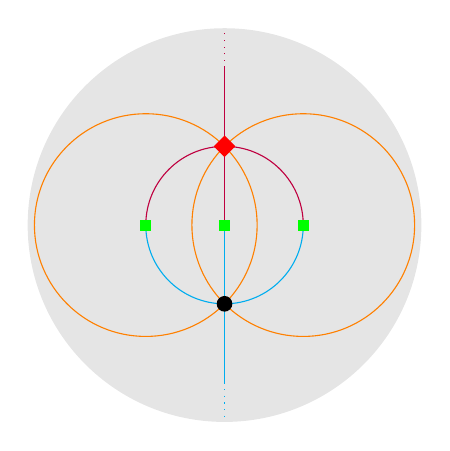
\begin{tikzpicture}
\fill[gray!20] (0,0) circle (2.5cm);

\coordinate (A) at (0,-1);
\coordinate (C) at (0,1);
\coordinate (B0) at (-1,0);
\coordinate (B1) at (0,0);
\coordinate (B2) at (1,0);

\draw[purple] (C) -- (B1);
\draw[purple] (C) -- (0,2);
\draw[purple,dotted] (0,2) -- (0,2.5);
\draw[purple] (-1,0) arc [start angle=180, end angle=90, radius=1];
\draw[purple] (1,0) arc [start angle=0, end angle=90, radius=1];

\draw[cyan] (A) -- (B1);
\draw[cyan] (A) -- (0,-2);
\draw[cyan,dotted] (0,-2) -- (0,-2.5);
\draw[cyan] (-1,0) arc [start angle=180, end angle=270, radius=1];
\draw[cyan] (1,0) arc [start angle=360, end angle=270, radius=1];

\draw[orange] (1,0) circle [radius=1.4142];
\draw[orange] (-1,0) circle [radius=1.4142];

\node[diamond,fill=red,inner sep=2pt] at (C) {};
\node[circle,fill=black,inner sep=2pt] at (A) {};
\foreach \x in {0,1,2}
\node[rectangle,fill=green,inner sep=2pt] at (B\x) {};

\end{tikzpicture}%
\end{document}
